\documentclass{DateStructure}

\SubjectName{交通咨询模拟问题}
\CollegeName{理学院}
\Major{信息与计算科学}
\GroupNumber{第十六组}
\StudentA{20071226}{童繁}{流程图}
\StudentB{20071227}{王瀚功}{数据}
\StudentC{20071228}{王赛豪}{文案}
\StudentD{20071229}{吴政豪}{调试}
\StudentE{20071230}{武琦}{代码}

\begin{document}
\makecover
\newpage
\thispagestyle{empty}
\tableofcontents   
\newpage
\setcounter{page}{1}  

\section{需求分析}
\begin{itemize}
\item[(1)]建立全国城市的公路网(包含高速公路、普通道路及其城市之间所需相应的时间和费用),编制汽车自驾出行的交通咨询程序,为旅客提供两种最优决策的交通咨询。
\item[(2)]提供对城市信息进行编辑(如添加、删除)的功能。
\item[(3)]提供两种最优决策:最快到达或最省钱到达。
\item[(4)]咨询以用户和计算机的对话方式进行。由用户输入起点、终点,最优决策原则,输出信息:最快需要多长时间或最少需要多少费用才能到达,并列出中间经过的城市和道路。
\end{itemize}

\section{项目亮点}
\begin{itemize}
\item[(1)]利用百度地图API爬取了392个省市的名字和经纬度,以及6万条两个城市驾车路线的时间和费用,具有现实参考意义。
\item[(2)]建立了密码登录(不显示输入)的管理员模式,实现管理员与用户的独立使用。
\item[(3)]用户在查询后可以实时显示出路线图,该图是基于百度地图API绘制的。
\item[(4)]建立了深色设置,用户可以根据现实时间自主调节白天或夜间模式,管理员的密码登录口隐藏在深色设置中。
\item[(5)]管理员可以在系统或文件中查看并修改相关信息,并实时保存。
\item[(6)]用户在选择查询后可以选择查看另一种方案。
\item[(7)]程序分割为三个库,使得项目的调用更加清晰合理。
\end{itemize}
\section{概要设计}
首先读取数据city.txt和city.csv,建立城市信息结构体及无向图的数据结构。\par
然后选择白天/夜间模式,管理员可以使用隐藏命令进入密码登录口,输入密码进入管理员模式,退出管理员模式时会自动回到用户模式。\par
用户在查询时,使用弗洛伊德算法,在用户输入起始城市和目标城市并选择了决策原则后,生成相应的最短路径。\par
整体的功能使用和输入合法性检验运用了C语言的goto函数,直到输入满足相应的选择后会执行其他程序。
\begin{figure}[H] 
\centering
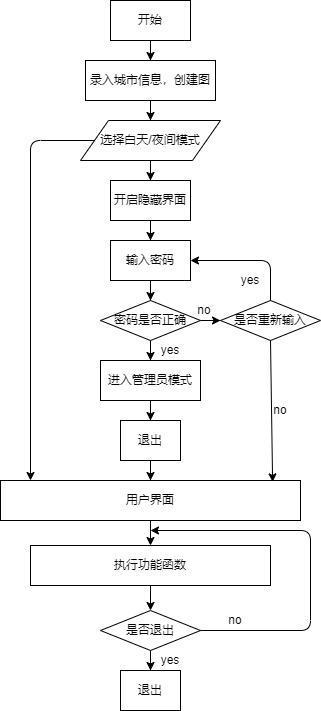
\includegraphics[width=250pt]{主函数.png}
\caption{主函数流程图}
\end{figure}
\section{详细设计}	
\subsection{定义}
运用两个邻接矩阵分别存储交通路线的时间和费用,将程序分割为city.c、admin.c和 function.c进行相关程序的编写。
\begin{figure}[H] 
\centering
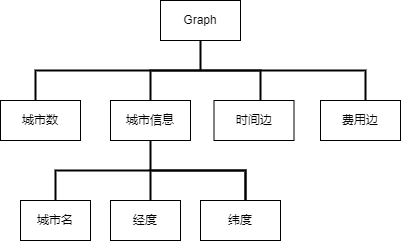
\includegraphics[width=300pt]{Graph.png}
\caption{数据结构示意图}
\end{figure}
\begin{figure}[H] 
\centering
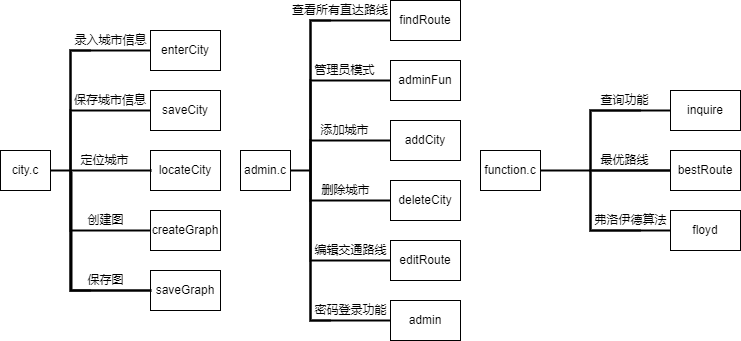
\includegraphics[width=400pt]{结构库.png}
\caption{函数结构示意图}
\end{figure}
\subsection{管理员模式}
在退出管理员模式前,保存城市信息和路线信息到city.txt和city.csv文件中。
\begin{figure}[H] 
\centering
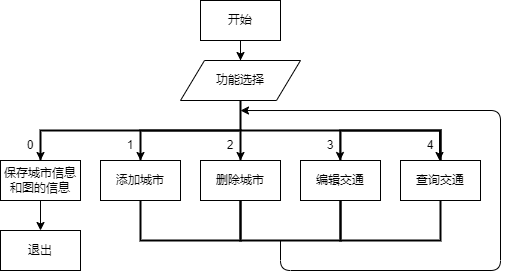
\includegraphics[width=300pt]{管理员模式流程.png}
\caption{管理员模式流程图}
\end{figure}
\subsection{用户模式}
关于路线图的绘制,首先将tmp.html复制为新的以“起始城市--目标城市”为文件名的html文件,然后通过C语言进行编写,最后使用C语言shellapi库的函数在浏览器打开文件。
\begin{figure}[H] 
\centering
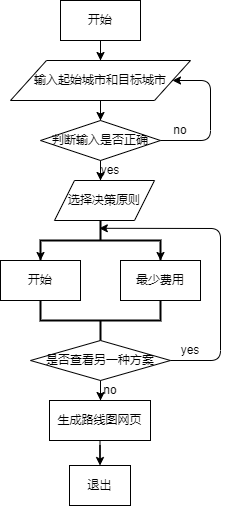
\includegraphics[width=150pt]{用户界面.png}
\caption{用户模式流程图}
\end{figure}
\newpage
\lstinputlisting[language=C]{./code/function.c}

\section{管理员手册}
管理员账号:33550336,密码:admin8128,登录口:496,数字都是完全数。
\subsection{管理员模式}
\begin{figure}[H] 
\centering
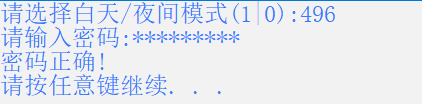
\includegraphics[width=300pt]{密码.png}
\caption{密码登录口}
\end{figure}
\begin{figure}[H] 
\centering
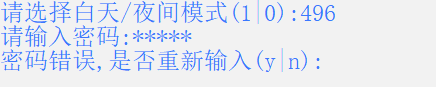
\includegraphics[width=300pt]{密码错误.png}
\caption{密码输入错误时}
\end{figure}
\begin{figure}[H] 
\centering
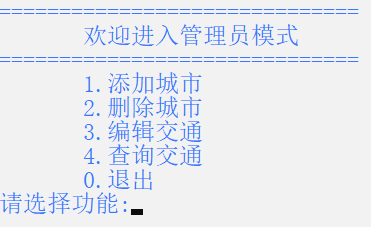
\includegraphics[width=300pt]{管理员模式.png}
\caption{管理员模式界面}
\end{figure}
\subsection{添加城市}
\begin{figure}[H] 
\centering
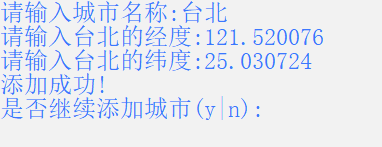
\includegraphics[width=300pt]{添加成功.png}
\caption{添加城市}
\end{figure}
\begin{figure}[H] 
\centering
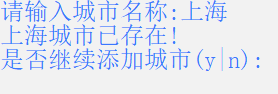
\includegraphics[width=300pt]{添加城市重复.png}
\caption{添加城市重复时}
\end{figure}
\subsection{删除城市}
\begin{figure}[H] 
\centering
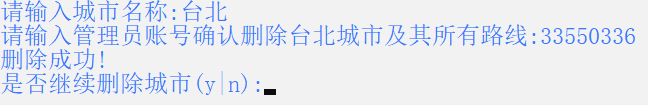
\includegraphics[width=300pt]{删除城市.png}
\caption{删除城市}
\end{figure}
\begin{figure}[H] 
\centering
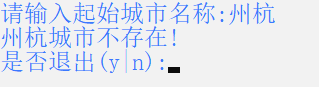
\includegraphics[width=300pt]{城市不存在.png}
\caption{城市不存在时}
\end{figure}
\subsection{编辑交通}
\begin{figure}[H] 
\centering
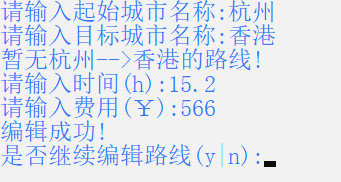
\includegraphics[width=300pt]{编辑交通1.png}
\caption{无路线时编辑交通}
\end{figure}
\begin{figure}[H] 
\centering
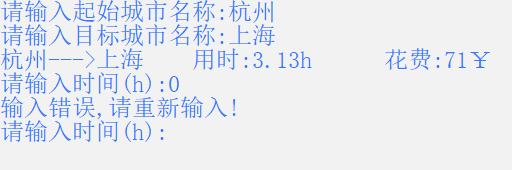
\includegraphics[width=300pt]{编辑交通2.png}
\caption{有路线时编辑交通}
\end{figure}
\subsection{查询路线}
管理员可以查询某个城市的所有直达路线。
\begin{figure}[H] 
\centering
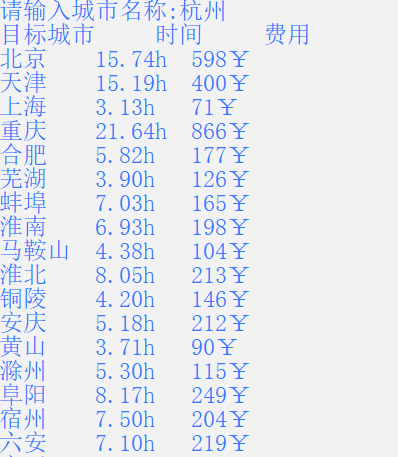
\includegraphics[width=300pt]{查询路线.png}
\caption{查询路线部分结果}
\end{figure}

\section{用户手册}
\begin{figure}[H] 
\centering
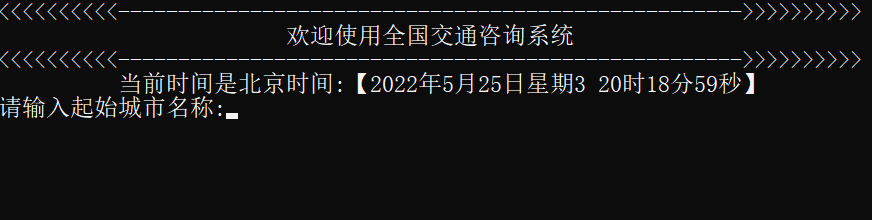
\includegraphics[width=300pt]{夜间模式.png}
\caption{夜间模式}
\end{figure}
\begin{figure}[H] 
\centering
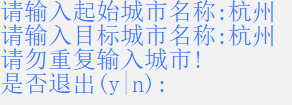
\includegraphics[width=250pt]{重复输入.png}
\caption{重复输入时}
\end{figure}
\begin{figure}[H] 
\centering
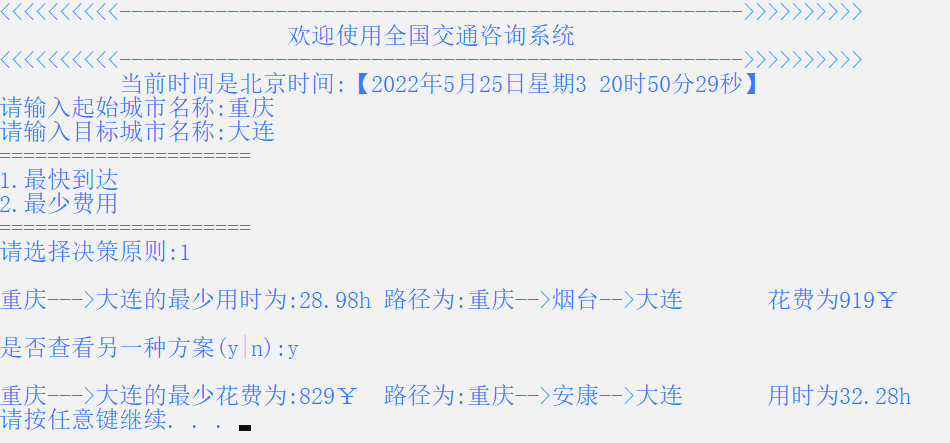
\includegraphics[width=300pt]{用户.png}
\caption{用户查询结果}
\end{figure}
\begin{figure}[H] 
\centering
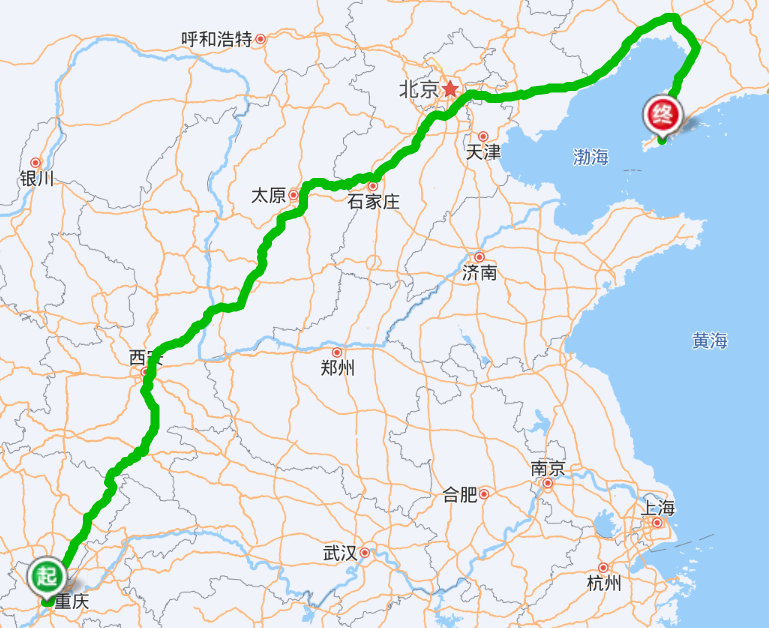
\includegraphics[width=300pt]{路线.png}
\caption{路线图(会自动在浏览器打开)}
\end{figure}
\begin{figure}[H] 
\centering
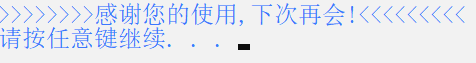
\includegraphics[width=300pt]{退出.png}
\caption{退出系统}
\end{figure}
\section{心得体会}
这次课程设计的心得体会通过实践我们的收获如下:\par
1.这次的交通咨询模拟课程设计,我们沿用了航空客运订票系统的文件存储函数和时间函数、家庭族谱的功能界面以及最小生成树问题的无向图数据结构,使得程序的编写方便快捷。\par
2.结合了之前课程设计的经验,提高了程序的鲁棒性。\par
3.学习了html文件的编写、Python基于API爬虫的原理和C语言shellapi库的应用。\par
4.这个项目是设计结构课程设计的最后一个项目,它结合了之前八次课程设计的Debug思想和编写范式,很好地体现了之前课程设计的收获。\par

\newpage 
\section{附录}
\subsection{definition.h}
\lstinputlisting[language=C]{./code/definition.h}
\subsection{city.c}
\lstinputlisting[language=C]{./code/city.c}
\subsection{admin.c}
\lstinputlisting[language=C]{./code/admin.c}
\subsection{function.c}
\lstinputlisting[language=C]{./code/function.c}
\subsection{main.c}
\lstinputlisting[language=C]{./code/main.c}
\subsection{baidu\_map\_api.py}
\lstinputlisting[language=Python]{./code/baidu_map_api.py}
\subsection{tmp.html}
\lstinputlisting{./code/tmp.html}

\end{document}
